\documentclass[10pt]{beamer}
\usepackage[spanish]{babel}
\selectlanguage{spanish} 
\usepackage[utf8]{inputenc}
\usepackage{default}
\usetheme{Montpellier}
%\usecolortheme{dolphin}
\usecolortheme{whale}
\usepackage{graphicx}
\usepackage{float} % supuestamente sirve para las tablas, con [H] se ponen en donde uno quiere
\restylefloat{table} % supuestamente sirve para las tablas, con [H] se ponen en donde uno quiere

\usepackage{subfig}    %para hacer figuras multiples
%\usepackage{hyperref}
\usepackage{cancel}

%\usepackage{wrapfig}
%\newcommand{\director}{Directores:\\Director name}

%\title%[Detecci\'on de Transitorios] % (optional, only for long titles)
%{Series Temporales en Galaxias}
%\subtitle{Detecci\'on de eventos transitorios en im\'agenes}
%\author[S\'anchez]%, Lares, Dom\'{i}nguez] % (optional, for multiple authors)
%{Bruno~S\'anchez\inst{1}\\% \and M.~Lares\inst{2} \and M.~Dom\'{i}nguez\inst{2}\inst{3}}
%\scriptsize{M.~Dom\'{i}nguez\inst{2}\inst{3} \and M.~Lares\inst{2}}}
%\institute[Universidad Nacional de C\'ordoba] % (optional)
%{
%  \inst{1}%
%  Observatorio Astron\'omico\\
%  Universidad Nacional de C\'ordoba
%  \and
%  \inst{2}%
%  Instituto de Astronom\'{i}a Te\'orica y Experimental \\
%  Universidad Nacional de C\'ordoba
%  \and
%  \inst{3}
  %Departamento Astrofisica??
%  University of Texas at Brownsville
%}

\begin{document}


\title[RB \& ML for transient astronomy]
{Real Bogus \& Machine Learning for transient astronomy}
%\subtitle{Gravitational arcs detection and real/bogus classification}
\institute{IATE - CONICET - Universidad Nacional de C\'ordoba (UNC)}
\titlegraphic{
\includegraphics[scale=0.8]{./images/vitraux_h90.png}}
\author{\begin{tabular}{r@{}l} 
Author:      & Bruno S\'anchez \\[1ex]   & Mariano Dom\'{i}nguez\\ & Marcelo Lares\\ & Mario D\'{i}az \\ & Mart\'{i}n Beroiz%Tania Tagliaferro  \\ & Carlos Valotto
\end{tabular}}
%\date{Date of Presentation}

%\begin{frame}
%  \titlepage
%\end{frame}
\frame{\titlepage}
%\begin{frame}
%\frametitle{Contents}
%\tableofcontents%[sectionstyle=show/hide, 
%sectionstyle=show/shaded]
%\end{frame}
%%%%%%%%%%%%%%%%%%%%%%%%%%%%%%%%%%%%%%%%%%%%%%%%%%%%%%%%%%%%%%%
%%%%%%%%%%%%%%%%%%%%%%%%%%%%%%%%%%%%%%%%%%%%%%%%%%%%%%%%%%%%%%%
\section{Introduction}
\frame{\tableofcontents[ 
    currentsection, 
    %hideothersections, 
    sectionstyle=show/hide, 
    sectionstyle=show/shaded, 
    ]}
%%%%%%%%%%%%%%%%%%%%%%%%%%%%%%%%%%%%%%%%%%%%%%%%%%%%%%%%%%%%%%%
\subsection{Astronomical Variability}
%%%%%%%%%%%%%%%%%%%%%%%%%%%%%%%%%%%%%%%%%%%%%%%%%%%%%%%%%%%%%%%
\begin{frame}
Variability studies in astronomy refer to the fluctuation of brightness over time
of an astronomical object.\\ 
\bigskip
We use variability studies for several things:
\begin{itemize}
\item Object classification 
\item NEO's studies
\item Stellar systems ($\alpha$ Cen)
\item Distance measures
\item Cosmology and cosmography
\end{itemize}
\end{frame}
%%%%%%%%%%%%%%%%%%%%%%%%%%%%%%%%%%%%%%%%%%%%%%%%%%%%%%%%%%%%%%%
\begin{frame}
There are several types of variability:
\begin{itemize}[<+->]
 \item Periodic Variability
 \only<1-1> {\begin{figure}[h] %%curva RRlyr
  %\includegraphics[width=2in,angle=-90]{./../../../tesis/manus/pics/curva_RRLyr.ps}
  \begin{center}
 \includegraphics[bb=0 0 806 559, width=0.7\textwidth]{./images/curva_RRLyr.png}
 % curva_RRLyr.png: 1119x776 pixel, 100dpi, 28.42x19.71 cm, bb=0 0 806 559
\end{center}

 % curva_RRLyr.ps: 595x841 pixel, 72dpi, 20.99x29.67 cm, bb=0 0 595 841
 \caption{\scriptsize{CRTSS light curve data for a RR Lyra star. }}
 %\label{fig:RRLyr}
\end{figure}}
 \item Transient Variability
 \only<2-2>{\begin{figure}[h]  %%curva ptf11kly
  %\includegraphics[width=3in]{./pics/ptf11kly.ps}
  \begin{center}
 \includegraphics[bb=0 0 1043 646, width=0.7\textwidth]{./images/ptf11kly.png}
 % ptf11kly.png: 1043x646 pixel, 72dpi, 36.79x22.79 cm, bb=0 0 1043 646
\end{center}
 % ptf11kly.ps: 1044x647 pixel, 72dpi, 36.83x22.82 cm, bb=0 0 1044 647
 \caption{\scriptsize{Supernova Type Ia lightcurve from PTF11kly. (PTF data).}}
%\label{fig:ptfkly_2}
\end{figure}
}
\only<3-3>{\begin{figure}
 \centering
 \includegraphics[width=0.7\textwidth,bb=0 0 93 49]{./images/ptf11kly.jpg}
 % ptf11kly.jpg: 1550x819 pixel, 1200dpi, 3.28x1.73 cm, bb=0 0 93 49
 \caption{\scriptsize{Supernova Type Ia (PTF11kly).}}
\end{figure}
}
\end{itemize}
\end{frame}
%%%%%%%%%%%%%%%%%%%%%%%%%%%%%%%%%%%%%%%%%%%%%%%%%%%%%%%%%%%%%%%
\subsection{A little about Gravitational Waves}
%%%%%%%%%%%%%%%%%%%%%%%%%%%%%%%%%%%%%%%%%%%%%%%%%%%%%%%%%%%%%%%
%%%%%%%%%%%%%%%%%%%%%%%%%%%%%%%%%%%%%%%%%%%%%%%%%%%%%%%%%%%%%%%
\begin{frame}
General Relativity (GR) admits on its equations the existence of \textbf{gravitational radiation}.\\ 
\bigskip
This Gravitational Waves (GW) would be \textbf{transversal waves}: induced perturbations arise in the 
perpendicular plane to the propagation direction.\\ \pause
\begin{figure}
 \centering
\begin{center}
 \includegraphics[bb=0 0 391 297, width=0.7\textwidth]{./images/Ondaviajandosobrecuerda2.jpg}
 % Ondaviajandosobrecuerda2.jpg: 391x297 pixel, 72dpi, 13.79x10.48 cm, bb=0 0 391 297
\end{center}
 % Ondaviajandosobrecuerda2.jpg: 391x297 pixel, 72dpi, 13.79x10.48 cm, bb=0 0 391 297
\end{figure}
\end{frame}
%%%%%%%%%%%%%%%%%%%%%%%%%%%%%%%%%%%%%%%%%%%%%%%%%%%%%%%%%%%%%%%
\begin{frame}
To detect this ALIGO is using Michelson interferometers\\ \pause 
For higher precision and sensibility this instruments need to be Km long
\begin{figure}%[H]  %michelson
   \centering
    \includegraphics[bb=0 0 342 263, width=0.45\textwidth]{./images/10-1.png}
     % 10-1.png: 342x263 pixel, 72dpi, 12.06x9.28 cm, bb=0 0 342 263
 \includegraphics[bb=0 0 642 343, width=0.45\textwidth]{./images/Hanford1.jpg}
 % Hanford1.jpg: 803x429 pixel, 90dpi, 22.66x12.11 cm, bb=0 0 642 343
     %\includegraphics[width=.45\textwidth,bb=14 14 657 358]{./pics/Hanford1.eps}
    %\caption{Interfer\'ometro de LIGO en Hanford}
   %\caption{\scriptsize{Esquema de un interfer\'ometro de Michelson.}}
  %\label{fig:Michelson}
  \end{figure}
\end{frame}
%%%%%%%%%%%%%%%%%%%%%%%%%%%%%%%%%%%%%%%%%%%%%%%%%%%%%%%%%%%%%%%
\begin{frame}
\begin{figure}%[h]  %%charliebrown
   %\includegraphics[bb=14 14 241 181, width=0.6\textwidth]{./pics/gw_detector.eps}
   \begin{center}
 \includegraphics[bb=0 0 227 166, width=0.7\textwidth]{./images/gw_detector.png}
 % gw_detector.png: 472x346 pixel, 150dpi, 7.99x5.86 cm, bb=0 0 227 166
  \caption{\scriptsize{Perturbations induced by GW (from \url{http://www.einstein-online.info/spotlights/gravWav}).}}
\end{center}
 %\label{fig:charliebrown}
 \end{figure}
\end{frame}
%%%%%%%%%%%%%%%%%%%%%%%%%%%%%%%%%%%%%%%%%%%%%%%%%%%%%%%%%%%%%%%
\begin{frame}
Localization errors of the candidates depends on N of detectors.
\begin{figure}%[h]
 \centering
 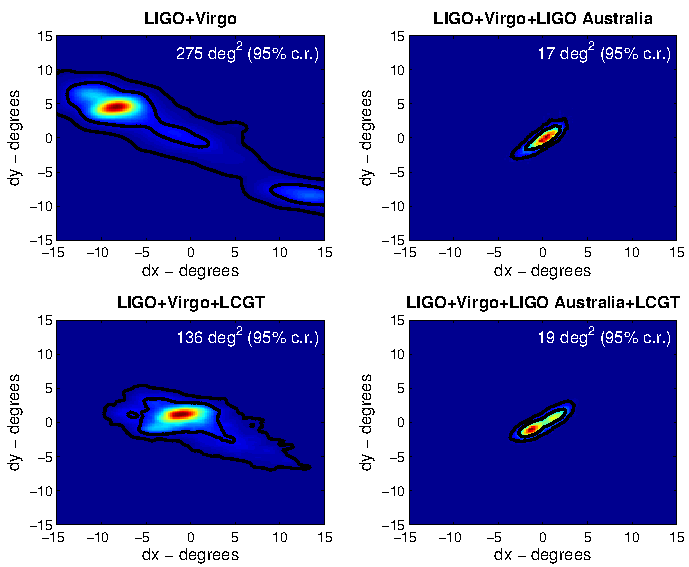
\includegraphics[width=0.7\textwidth]{./images/fig2.png}
 % fig2.eps: 0x0 pixel, 300dpi, 0.00x0.00 cm, bb=   52   197   548   605
 \caption{\scriptsize{Sky localization of a low-limit SNR.}} 
 %Las lineas negras solidas indican una regi\'on con una confidencia del 68\% y 95\%, y 
 %sobre cada figura se muestra que red particular se utiliz\'o.}
 %\label{fig:skyerror1}
\end{figure}
\end{frame}
%%%%%%%%%%%%%%%%%%%%%%%%%%%%%%%%%%%%%%%%%%%%%%%%%%%%%%%%%%%%%%%
\begin{frame}
So ALIGO needs confirmation of candidates by a independent method.\\
\pause
This independent tracer are the \textbf{Compact Object Mergers}.\\
This objects would produce bursts of EM radiation,
(the so called ``smoking gun'').\\
In the optical range we find the Kilonova event.
\begin{figure}
 %\centering
 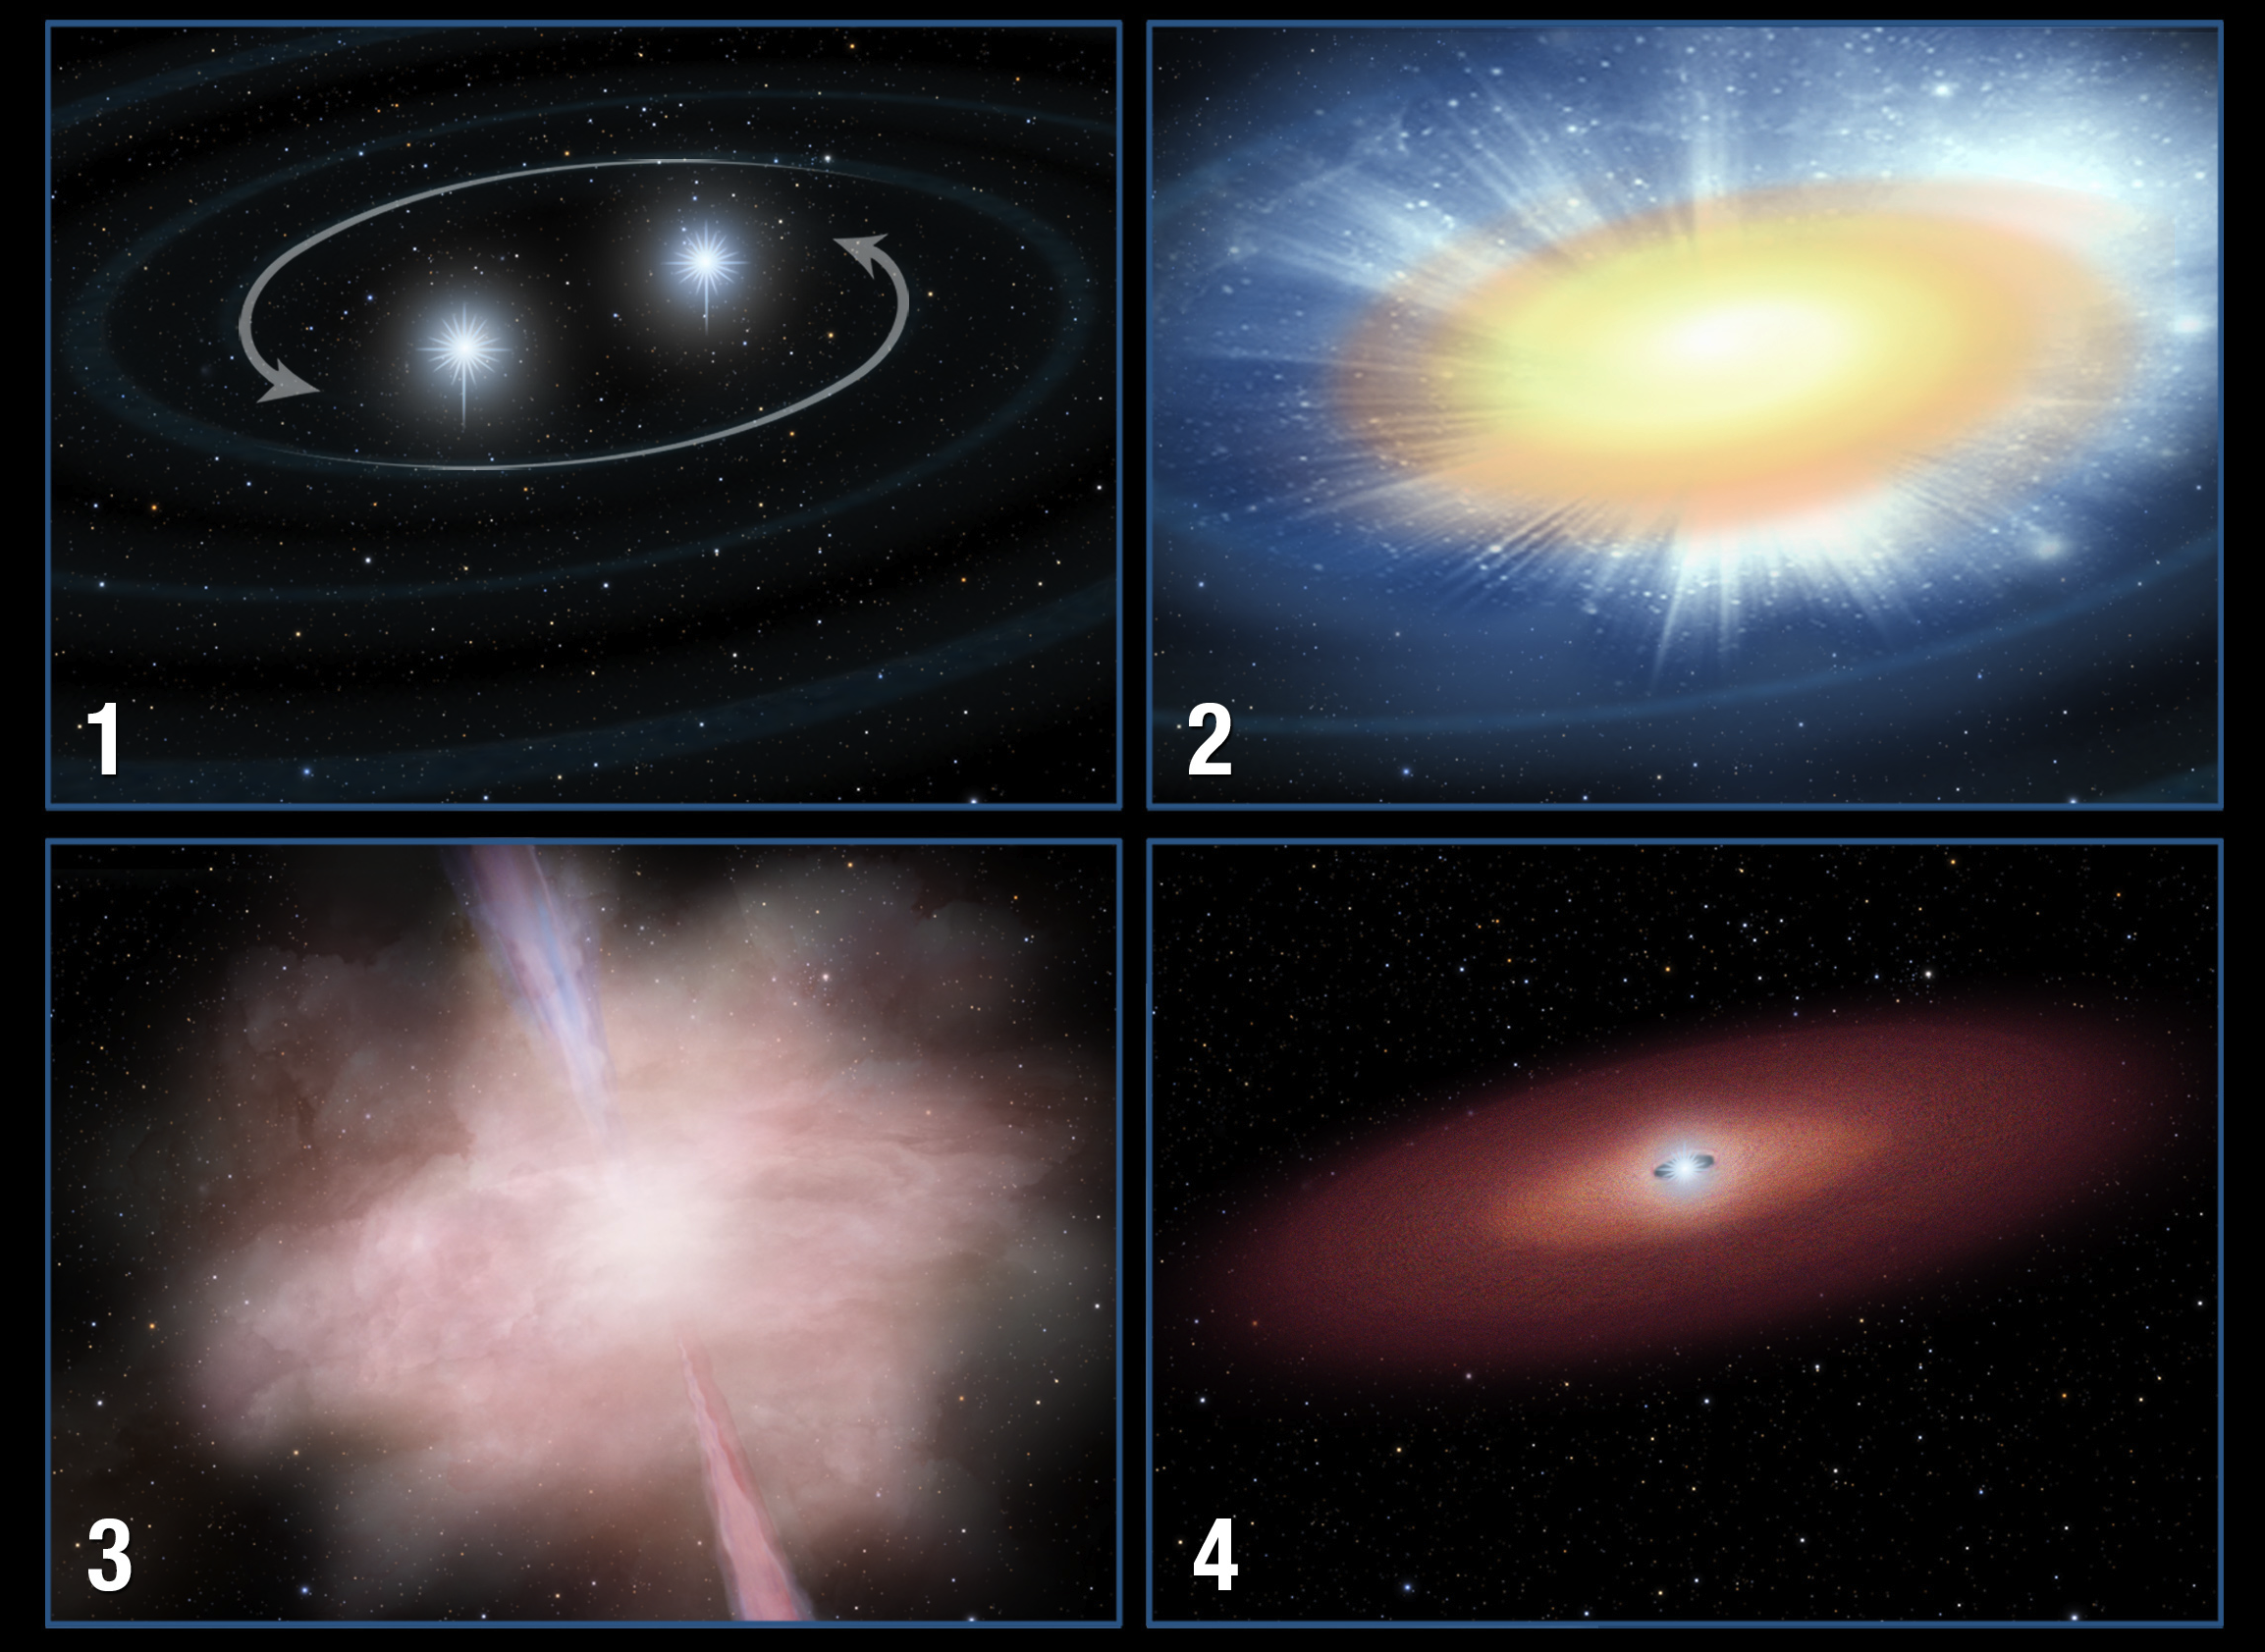
\includegraphics[width=0.45\textwidth,bb=0 0 2307 1683]{./images/merger_model.png}
 % merger_model.ps: 2307x1683 pixel, 72dpi, 81.39x59.37 cm, bb=0 0 2307 1683
 \caption{\scriptsize{Compact object merger cartoon}}
 %: (1) Sistema binario de estrellas de neutrones; 
 %(2) concluida la etapa de acercamiento en espiral los objetos toman contacto; 
 %(3) los objetos se fusionan disparando un jet en la direcci\'on perpendicular al plano orbital y expulsando material que emite radiaci\'on casi isotr\'opicamente; 
 %(4) el material eyectado decae radioactivamente y se apaga formando un disco. Extra\'{i}do de \url{http://www.einstein-online.info/spotlights/gravWav}.}}
 %\label{fig:merger}
\end{figure}
\end{frame}
%%%%%%%%%%%%%%%%%%%%%%%%%%%%%%%%%%%%%%%%%%%%%%%%%%%%%%%%%%%%%%%
\subsection{TOROS/TORITOS \& Astronomical imaging}
%%%%%%%%%%%%%%%%%%%%%%%%%%%%%%%%%%%%%%%%%%%%%%%%%%%%%%%%%%%%%%%
%%%%%%%%%%%%%%%%%%%%%%%%%%%%%%%%%%%%%%%%%%%%%%%%%%%%%%%%%%%%%%%
\begin{frame}
 There is only one observed Kilonova.\\ 
 \pause
 So... what is needed to catch a Kilonova??
 \begin{itemize}[<+->]
  \item Telescope time
  \item Great number of observations
  \item Be able to detect short timescale variability
  \item High-speed data processing 
 \end{itemize}
 \pause
 Project TOROS - TORITOS
\begin{figure}
 \centering
 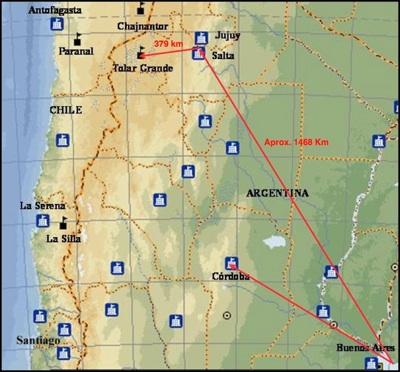
\includegraphics[bb=0 0 400 372, width=0.3\textwidth]{./images/Site.jpg}
 % Site.jpg: 400x372 pixel, 72dpi, 14.11x13.12 cm, bb=0 0 400 372
 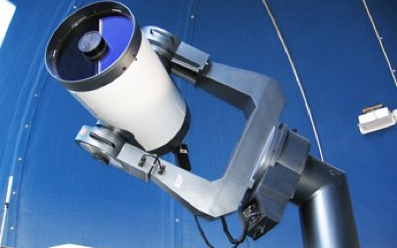
\includegraphics[bb=0 0 159 99, width=0.45\textwidth]{./images/toritos_1.png}
 % toritos_1.png: 397x248 pixel, 180dpi, 5.60x3.50 cm, bb=0 0 159 99
\end{figure}
\end{frame}
%%%%%%%%%%%%%%%%%%%%%%%%%%%%%%%%%%%%%%%%%%%%%%%%%%%%%%%%%%%%%%%
\begin{frame}\frametitle{Image analysis}
There are two different techniques:
\begin{itemize}
 \item Aperture photometry \pause
 \begin{itemize}
  \item Calculates the energy received on a given area of the image %\pause
  \item $m_1 - m_2 = -2.5 log_{10}\left(\frac{E_1}{E_2}\right)$ %\pause
\begin{figure}
  \begin{center}
 \includegraphics[width=0.4\textwidth]{./images/apertures.png}
 % apertures.png: 680x472 pixel, 72dpi, 23.99x16.65 cm, bb=0 0 680 472
\end{center}
\end{figure}
 \end{itemize}
 \item Difference Image Analysis \pause
 \begin{itemize}
  \item It is like ``fancy substracting'' two images%\pause
 \end{itemize}
\end{itemize}
\end{frame}
%%%%%%%%%%%%%%%%%%%%%%%%%%%%%%%%%%%%%%%%%%%%%%%%%%%%%%%%%%%%%%%
\begin{frame}\frametitle{Image analysis}
 Our main approach relies on the second technique. \\
 \pause
 In a perfect substraction we would be having a image like this:
 \begin{center}
 \includegraphics[width=0.7\textwidth,bb=0 0 41 28,keepaspectratio=true]{./images/ds9.png}
 % ds9.tif: 680x472 pixel, 1200dpi, 1.44x1.00 cm, bb=0 0 41 28
\end{center}
\pause
In this example there are not transients.
Althoug we can see some random noise resembling stars.
\end{frame}
%%%%%%%%%%%%%%%%%%%%%%%%%%%%%%%%%%%%%%%%%%%%%%%%%%%%%%%%%%%%%%%
\begin{frame}\frametitle{Image analysis}
This image presents transients:
\begin{center}
 \includegraphics[width=0.7\textwidth,bb=0 0 41 28,keepaspectratio=true]{./images/ds9resta.png}
 % ds9resta.tif: 680x472 pixel, 1200dpi, 1.44x1.00 cm, bb=0 0 41 28
\end{center}
\pause
But this two are fake images.
\end{frame}
%%%%%%%%%%%%%%%%%%%%%%%%%%%%%%%%%%%%%%%%%%%%%%%%%%%%%%%%%%%%%%%
\begin{frame}\frametitle{Image analysis}
 This is an actual subtraction from real data:
 \begin{center}
 \includegraphics[width=0.9\textwidth,bb=0 0 41 28,keepaspectratio=true]{./images/ds9restareal.png}
 % ds9resta.tif: 680x472 pixel, 1200dpi, 1.44x1.00 cm, bb=0 0 41 28
\end{center}
\end{frame}
%%%%%%%%%%%%%%%%%%%%%%%%%%%%%%%%%%%%%%%%%%%%%%%%%%%%%%%%%%%%%%%
\begin{frame}\frametitle{Image analysis}
 In order to clean this kind of data we apply Statistical Learning methods, 
 also called Machine Learning methods.\\ \bigskip
 \pause 
 The classificator that separates false from real candidates is called Real-Bogus
\end{frame}

%%%%%%%%%%%%%%%%%%%%%%%%%%%%%%%%%%%%%%%%%%%%%%%%%%%%%%%%%%%%%%%
\section{Real/Bogus: A Machine Learning solution}
%%%%%%%%%%%%%%%%%%%%%%%%%%%%%%%%%%%%%%%%%%%%%%%%%%%%%%%%%%%%%%%
\frame{\tableofcontents[ 
    currentsection, 
    %hideothersections, 
    sectionstyle=show/hide, 
    sectionstyle=show/shaded, 
    ]}
%%%%%%%%%%%%%%%%%%%%%%%%%%%%%%%%%%%%%%%%%%%%%%%%%%%%%%%%%%%%%%%
\subsection{What is Machine Learning?} %the concept of a learning algorithm.
%%%%%%%%%%%%%%%%%%%%%%%%%%%%%%%%%%%%%%%%%%%%%%%%%%%%%%%%%%%%%%%
\begin{frame} \frametitle{Statistical Learning}
First of all: \textit{What is machine learning?}\\ \pause
\centering
\textbf{Supervised learning}
 \begin{figure}
 \includegraphics[bb=0 0 3506 2549,scale=0.062]{./images/supervised.png}
 % supervised.png: 3506x2549 pixel, 72dpi, 123.67x89.91 cm, bb=0 0 3506 2549
\end{figure}
\end{frame}
%%%%%%%%%%%%%%%%%%%%%%%%%%%%%%%%%%%%%%%%%%%%%%%%%%%%%%%%%%%%%%%
\begin{frame}\frametitle{Statistical learning}
 The machine learning jargon includes different terms:
 \begin{itemize}[<+->]
  \item \textbf{Objective class}: is the information we need to predict with a ML algorithm. It can be 
  numeric, or categoric. The simplest is a binary objective class, such as R-B problem.
  \item \textbf{Instances}: this are basically data points. Also called ``examples'', and they conform the
  datasets for training and testing stage.
  \item \textbf{Features}: are the measurables that we can extract from a given instance. Also represented as a vector
  $\vec{f}_i$ for the instance number $i$. These features can be also categoric or numeric. 
  \item \textbf{Labeled data}: these data are instances that we are going to use as training set. Labeled means that 
  you already know which is the true class for each instance.
 \end{itemize}
\end{frame}

%%%%%%%%%%%%%%%%%%%%%%%%%%%%%%%%%%%%%%%%%%%%%%%%%%%%%%%%%%%%%%%
\begin{frame} \frametitle{Statistical Learning}
\begin{columns}
 \begin{column}{0.3\textwidth}
 So a dataset with a correct labeling of different objects
 is needed to obtain a classificator.\\
 This can be achieved for example by using citizen science:
 \url{http://toros-dev.no-ip.org}
 \end{column}
 \begin{column}{0.7\textwidth}
 \begin{center}
 \includegraphics[width=1.0\textwidth,keepaspectratio=True]{./images/Winnow.png}
 % Winnow - Training Page 2015-07-17 00-37-38.png: 728x600 pixel, 72dpi, 25.68x21.17 cm, bb=0 0 728 600
\end{center}
\end{column}
\end{columns}

\end{frame}

%%%%%%%%%%%%%%%%%%%%%%%%%%%%%%%%%%%%%%%%%%%%%%%%%%%%%%%%%%%%%%%
\subsection{Algorithms implemented} %the concept of a learning algorithm.
%%%%%%%%%%%%%%%%%%%%%%%%%%%%%%%%%%%%%%%%%%%%%%%%%%%%%%%%%%%%%%%
%%%%%%%%%%%%%%%%%%%%%%%%%%%%%%%%%%%%%%%%%%%%%%%%%%%%%%%%%%%%%%%%
\begin{frame} \frametitle{Algorithms implemented}
Implemented three algorithms from ML:
\begin{itemize}%[<+->]
 \item \textbf{Naive Bayes}
 \only<3>{Uses the Bayes's theorem in order to estimate probabilities of belonging to different classes. \\ 
 %\begin{displaymath}
 % P(A|B)P(B) = P(B|A)P(A)
 %\end{displaymath}
%This is a symetrical relationship between two random variables, and
%its ocurrence probabilities.
%Using this it can be estimated a probability of belonging to 
%a given class for a new observation, 
%using the information given in the previous experience:
\begin{displaymath}
 P(c=R|\vec{f_i}) = \frac{P(\vec{f_i}|c=R)P(c=R)}{P(\vec{f_i})}
\end{displaymath}
}
 \item  \textbf{Logistic Regression}
 \only<4>{This algorithm assumes that probabilities of belonging to
 a given class can be linearly interpolated after a simple transformation:
 \begin{displaymath}
  logi(p_R) = \ln(\frac{p_R}{1-p_R}) = \alpha + \beta \times \vec{f}_i
 \end{displaymath}
%where $logi$ is the \textit{logistic function}, $p_i$ the probability of
%belonging to a given class, and again $\vec{f}$ is the features of each data point.
}
\item \textbf{Random Forest}
\only<5>{This algorithm works growing decision trees
by using two parameters: $N_{tree}$ the number of 
decision trees to be trained, and $N_f$ the number of random 
features on each tree.\\ 
After training the decision is made taking into account all the trees votes.}
\end{itemize}
\end{frame}
%%%%%%%%%%%%%%%%%%%%%%%%%%%%%%%%%%%%%%%%%%%%%%%%%%%%%%%%%%%%%%%
%%%%%%%%%%%%%%%%%%%%%%%%%%%%%%%%%%%%%%%%%%%%%%%%%%%%%%%%%%%%%%%
\subsection{Real/Bogus implemented on simulated data}
%%%%%%%%%%%%%%%%%%%%%%%%%%%%%%%%%%%%%%%%%%%%%%%%%%%%%%%%%%%%%%%
%%%%%%%%%%%%%%%%%%%%%%%%%%%%%%%%%%%%%%%%%%%%%%%%%%%%%%%%%%%%%%%
%%%%%%%lots of things missing here commented
%%%%%%%%%%%%%%%%%%%%%%%%%%%%%%%%%%%%%%%%%%%%%%%%%%%%%%%%%%%%%%%
%%%%%%%%%%%%%%%%%%%%%%%%%%%%%%%%%%%%%%%%%%%%%%%%%%%%%%%%%%%%%%%
\begin{frame}\frametitle{Constructing traning dataset}
We simulated data giving a balanced set of 9202 \textit{bogus} y 9120 \textit{reals}.
%\pause
\begin{figure}
 \centering
 \includegraphics[scale=1]{../../Doctorado/codigos/scipycodes/image-simulation-and-analysis/bogus/obj_002.png}
 \includegraphics[scale=1]{../../Doctorado/codigos/scipycodes/image-simulation-and-analysis/bogus/obj_011.png}
 \includegraphics[scale=1]{../../Doctorado/codigos/scipycodes/image-simulation-and-analysis/bogus/obj_013.png}
 \includegraphics[scale=1]{../../Doctorado/codigos/scipycodes/image-simulation-and-analysis/bogus/obj_018.png}
 % obj_002.png: 64x64 pixel, 72dpi, 2.26x2.26 cm, bb=0 0 64 64
 \caption{Stamps of bogus simulated objects.}
 \label{fig:bogus}
\end{figure}
\begin{figure}
 \centering
 \includegraphics[scale=1]{../../Doctorado/codigos/scipycodes/image-simulation-and-analysis/real/robj_0025.png}
 \includegraphics[scale=1]{../../Doctorado/codigos/scipycodes/image-simulation-and-analysis/real/robj_0041.png}
 \includegraphics[scale=1]{../../Doctorado/codigos/scipycodes/image-simulation-and-analysis/real/robj_0040.png}
 \includegraphics[scale=1]{../../Doctorado/codigos/scipycodes/image-simulation-and-analysis/real/robj_0115.png}
 % obj_002.png: 64x64 pixel, 72dpi, 2.26x2.26 cm, bb=0 0 64 64
 \caption{Simulated real objects.}
 \label{fig:reals}
\end{figure}
\end{frame}
%%%%%%%%%%%%%%%%%%%%%%%%%%%%%%%%%%%%%%%%%%%%%%%%%%%%%%%%%%%%%%%
\begin{frame}\frametitle{Procedure}
\begin{itemize}[<+->]
 \item We implemented a \textbf{vectorizer}, which simply uses the image pixel data
and extracts a huge set of features -it can extract almost 3000 features-, 
and we used a reduced \textbf{set of 1028 features}.
 \item After that we implemented \textbf{WEKA Explorer suit} to analyze the data.
It contains several standard ML tools, including \textbf{feature selection}.
 \item From this tools we employed two feature selection routines: PCA, and 
CfSubsetEval from Hall (1998). This two algorithms reduce the 1028
set of features in order to discard interdependencies.
 \item PCA threw 310 principal components, giving also the transformation matrix, and
features vectors already projected into the PCA space.
 \item The second method found that the best features were 39, and so we used this subsample to 
train the classificators.
\end{itemize}
\end{frame}
%%%%%%%%%%%%%%%%%%%%%%%%%%%%%%%%%%%%%%%%%%%%%%%%%%%%%%%%%%%%%%%
\subsection{The construction of Figure of Merit}
%%%%%%%%%%%%%%%%%%%%%%%%%%%%%%%%%%%%%%%%%%%%%%%%%%%%%%%%%%%%%%%
\begin{frame}\frametitle{FOM}
 We call Figure of Merit to a set of estimators of a certain test perfomance.
During every decistion process we deal with two possible errors: 
%{%
%\newcommand{\mc}[3]{\multicolumn{#1}{#2}{#3}}
\begin{center}
\begin{tabular}{|c|c|l|}
\hline
- & \multicolumn{2}{c|}{Desition}\\
\hline \hline
Actual State & Reject $H_0$ & \multicolumn{1}{c|}{No reject $H_0$}\\
\hline
$H_0$ True & Type I Error & \multicolumn{1}{c|}{Correct}\\
\hline
$H_0$ False & Correct & \multicolumn{1}{c|}{Type II Error}\\
\hline
\end{tabular}
\end{center}
This also represents the so called ``Confusion Matrix''
%}%
\end{frame}
%%%%%%%%%%%%%%%%%%%%%%%%%%%%%%%%%%%%%%%%%%%%%%%%%%%%%%%%%%%%%%%
\begin{frame} \frametitle{FOM}
 Some common quantities that measure the perfomance of a test are FDR, TPR, y FPR.
\begin{itemize}
 \item FDR \textit{False Discovery Rate} is the probability of making a Type I 
 mistake, given that you already rejected $H_0$
 \item TPR \textit{True Positive Rate}) is the probability of rejecting 
$H_0$ given that it is false, or 1- the probability of making a Type I mistake
\item FPR (o \textit{False Positive Rate}) is the probability 
 of making a Type II mistake
\end{itemize}
\end{frame}
%%%%%%%%%%%%%%%%%%%%%%%%%%%%%%%%%%%%%%%%%%%%%%%%%%%%%%%%%%%%%%%
\begin{frame} \frametitle{FOM}
 \begin{columns}[T]
\begin{column}{0.48\textwidth}\bigskip
There is a compromise between FPR and TPR.\\
This compromise serves the preferences of the test's user for the 
confidence
 This curve is called \textit{Receiver Operating Characteristic} or ROC.\\ 
  The most used estimator is called AUC for \textit{Area under the Curve}
 \end{column}
 \begin{column}{0.55\textwidth}
 \begin{figure}
 \centering
 \includegraphics[width=\textwidth]{./images/ROC.png}
 % ROC.ps: 504x504 pixel, 72dpi, 17.78x17.78 cm, bb=0 0 504 504
 \caption{\scriptsize{Curva ROC}}
 %\label{fig:roc}
\end{figure}
\end{column}
 \end{columns}
\end{frame}
%%%%%%%%%%%%%%%%%%%%%%%%%%%%%%%%%%%%%%%%%%%%%%%%%%%%%%%%%%%%%%%
\begin{frame} \frametitle{FOM}
\begin{columns}
 \begin{column}{0.45\textwidth}
 There are others FoM for different purpouses.
 FPR and TPR can be ``fooled'' in the presence of an unbalanced
 training set.\\
 $N_B \sim \epsilon\times N_R$ \\
 In some data sets $\epsilon$ goes from 30 to 100.
 So the training set is unbalanced.\\
 \end{column}
 \begin{column}{0.5\textwidth}
$Precision = P(Y=1|\hat{Y} = 1)$ \\
$Recall = P(\hat{Y} = 1 | Y=1)$ \\
$Specificity = P(\hat{Y} = 0 | Y=0)$ \\
\bigskip
 Recall and Specificity relie on conditionals from 
 the \textbf{true class labels}. \\
 Precision relies on conditionals from 
 \textbf{your estimate} of the true class label.
\end{column}

 \end{columns}
\end{frame}
%%%%%%%%%%%%%%%%%%%%%%%%%%%%%%%%%%%%%%%%%%%%%%%%%%%%%%%%%%%%%%%
\begin{frame} \frametitle{FOM}
\begin{center}
 \includegraphics[width=\textwidth,bb=0 0 1310 648]{./images/mzwkk.png}
 % mzwkk.png: 1310x648 pixel, 72dpi, 46.21x22.86 cm, bb=0 0 1310 648
\end{center}
\end{frame}
%%%%%%%%%%%%%%%%%%%%%%%%%%%%%%%%%%%%%%%%%%%%%%%%%%%%%%%%%%%%%%%
\begin{frame} \frametitle{FOM}
\begin{columns}
\begin{column}{0.5\textwidth}
 \begin{figure}
 \centering
 \includegraphics[width=1.\textwidth]{./images/precisionrecall1.png}
 % Precisionrecall.svg.png: 320x582 pixel, 72dpi, 11.29x20.53 cm, bb=0 0 320 582
% \caption{\scriptsize{by Walber. Licensed under CC BY-SA 4.0 via Wikimedia Commons}}
\end{figure}
\end{column}
\begin{column}{0.5\textwidth}
 \begin{figure}
 \centering
 \includegraphics[width=1.1\textwidth]{./images/precisionrecall2.png}
 % Precisionrecall.svg.png: 320x582 pixel, 72dpi, 11.29x20.53 cm, bb=0 0 320 582
% \caption{\scriptsize{by Walber. Licensed under CC BY-SA 4.0 via Wikimedia Commons}}
\end{figure}
\end{column}
\end{columns}
\end{frame}
%%%%%%%%%%%%%%%%%%%%%%%%%%%%%%%%%%%%%%%%%%%%%%%%%%%%%%%%%%%%%%%
\begin{frame}\frametitle{K-fold cross validation}
 The perfomance was calculated using K-Fold Cross Validation algorithm, 
 which divides the dataset into \textbf{K slices randomly sampled} and trains
 in K-1 folds while testing over the fold unused. 
 \begin{figure}
 \includegraphics[width=0.6\textwidth,bb=0 0 300 137,keepaspectratio=true]{./images/k-fold.jpg}
 % k-fold.jpg: 471x215 pixel, 113dpi, 10.59x4.83 cm, bb=0 0 300 137
\end{figure}
 %\pause
 Since this can be performed K times, the testing gives K measures, 
 and then those are combined to extract the TPR and FPR statistics.
\end{frame}
%%%%%%%%%%%%%%%%%%%%%%%%%%%%%%%%%%%%%%%%%%%%%%%%%%%%%%%%%%%%%%%
%%%%%%%%%%%%%%%%%%%%%%%%%%%%%%%%%%%%%%%%%%%%%%%%%%%%%%%%%%%%%%%
\begin{frame}[c, squeeze] \frametitle{Complete sample results}
\begin{columns}
\begin{column}{0.3\textwidth}
\begin{center}
\textbf{Naive Bayes} 
\begin{figure}
 \includegraphics[bb=0 0 512 512,scale=0.16]{./images/RB_fullset_NB.png}
 % RB_fullset_NB.png: 512x512 pixel, 72dpi, 18.06x18.06 cm, bb=0 0 512 512
\end{figure}
\end{center}
\end{column}
\begin{column}{0.3\textwidth}
\begin{center}
\textbf{Random Forest}
\begin{figure}
 \includegraphics[bb=0 0 512 512,scale=0.16]{./images/RB_fullset_RF.png}
 % RB_fullset_RF.png: 512x512 pixel, 72dpi, 18.06x18.06 cm, bb=0 0 512 512
\end{figure}

\end{center}
\end{column}
\begin{column}{0.34\textwidth}
 \begin{figure}
 \includegraphics[bb=0 0 480 480,scale=0.249]{./images/full_sample_RB.png}
 % full_sample_RB.png: 480x480 pixel, 72dpi, 16.93x16.93 cm, bb=0 0 480 480
\end{figure}
\end{column}
\end{columns}
\end{frame}
%%%%%%%%%%%%%%%%%%%%%%%%%%%%%%%%%%%%%%%%%%%%%%%%%%%%%%%%%%%%%%%
\begin{frame}[c, squeeze] \frametitle{PCA transformed sample results}
%\only<1>{
\scriptsize
 \begin{columns}
\begin{column}{0.5\textwidth}
\begin{center}
\textbf{Naive Bayes} 
\begin{figure}
 \includegraphics[bb=0 0 512 512,scale=0.136]{./images/RB_PCAset_NB.png}
 % RB_PCAset_NB.png: 512x512 pixel, 72dpi, 18.06x18.06 cm, bb=0 0 512 512
\end{figure}
\textbf{Logistic Regression} %results for PCA features:\pause
\begin{figure}
 \includegraphics[bb=0 0 512 512,scale=0.136]{./images/RB_PCAset_LR.png}
 % RB_PCAset_LR.png: 512x512 pixel, 72dpi, 18.06x18.06 cm, bb=0 0 512 512
\end{figure}
\end{center}
\end{column}

\begin{column}{0.5\textwidth}
\begin{center}
\textbf{Random Forest}% results for PCA features:\pause
\begin{figure}
 \includegraphics[bb=0 0 512 512,scale=0.136]{./images/RB_PCAset_RF.png}
 % RB_PCAset_RF.png: 512x512 pixel, 72dpi, 18.06x18.06 cm, bb=0 0 512 512
\end{figure}

%\end{center}
%\end{column}
% \end{columns}}
% \only<2>{
 \begin{figure}
 \centering
 \includegraphics[bb=0 0 480 480,scale=0.2]{./images/PCA_RB.png}
 % PCA_RB.png: 480x480 pixel, 72dpi, 16.93x16.93 cm, bb=0 0 480 480
\end{figure}
%}
\end{center}
\end{column}
\end{columns}
\end{frame}
%%%%%%%%%%%%%%%%%%%%%%%%%%%%%%%%%%%%%%%%%%%%%%%%%%%%%%%%%%%%%%%
\begin{frame}[c, squeeze] \frametitle{Cfs selected features results}
 \scriptsize
 \begin{columns}\begin{column}{0.5\textwidth}
\begin{center}
 \textbf{Naive Bayes} 
 \begin{figure}
 \centering
 \includegraphics[bb=0 0 512 512,scale=0.14]{./images/RB_Cfsset_NB.png}
 % RB_Cfsset_NB.png: 512x512 pixel, 72dpi, 18.06x18.06 cm, bb=0 0 512 512
\end{figure}

\textbf{Logistic Regression} %results for best features:\pause
\begin{figure}
 \centering
 \includegraphics[bb=0 0 512 512,scale=0.14]{./images/RB_Cfsset_LR.png}
 % RB_Cfsset_LR.png: 512x512 pixel, 72dpi, 18.06x18.06 cm, bb=0 0 512 512
\end{figure}
\end{center}
\end{column}
\begin{column}{0.5\textwidth}
\begin{center}
\textbf{Random Forest} %results for best features:\pause
\begin{figure}
 \centering
 \includegraphics[bb=0 0 512 512,scale=0.14]{./images/RB_Cfsset_RF.png}
 % RB_Cfsset_RF.png: 512x512 pixel, 72dpi, 18.06x18.06 cm, bb=0 0 512 512
\end{figure}
\begin{figure}
 \centering
 \includegraphics[bb=0 0 480 480,scale=0.2]{./images/Cfs_RB.png}
 % Cfs_RB.png: 480x480 pixel, 72dpi, 16.93x16.93 cm, bb=0 0 480 480
\end{figure}
\end{center} 
\end{column}
\end{columns}
\end{frame}

%%%%%%%%%%%%%%%%%%%%%%%%%%%%%%%%%%%%%%%%%%%%%%%%%%%%%%%%%%%%%%%
%%%%%%%%%%%%%%%%%%%%%%%%%%%%%%%%%%%%%%%%%%%%%%%%%%%%%%%%%%%%%%%
\section{Conclusions \& future work}
%%%%%%%%%%%%%%%%%%%%%%%%%%%%%%%%%%%%%%%%%%%%%%%%%%%%%%%%%%%%%%%
\frame{\tableofcontents[ 
    currentsection, 
    %hideothersections, 
    sectionstyle=show/hide, 
    sectionstyle=show/shaded, 
    ]}
%%%%%%%%%%%%%%%%%%%%%%%%%%%%%%%%%%%%%%%%%%%%%%%%%%%%%%%%%%%%%%%
\begin{frame}%[allowframebreaks]
\frametitle{Summary and conclusions}
\begin{itemize}[<+->]
\item We implemented Machine Learning algorithms for classification in astronomical
images, using a vectorizer and feature selection methods.
\item The results showed a powerful tool that can be employed easily and with high confidence.
\item The flexibility of these methods make them exceptionally expandable to other situations.
\end{itemize}
\end{frame}
%%%%%%%%%%%%%%%%%%%%%%%%%%%%%%%%%%%%%%%%%%%%%%%%%%%%%%%%%%%%%%%
\begin{frame}\frametitle{Future work}
 \begin{itemize}
  \item Use this for TOROS/TORITOS (deployment on spring).
  \item Classify light curves
\end{itemize}
\begin{center}
\pause
\textbf{PREGUNTAS?? :D}
\end{center}
\end{frame}
%%%%%%%%%%%%%%%%%%%%%%%%%%%%%%%%%%%%%%%%%%%%%%%%%%%%%%%%%%%%%%%
%%%%%%%%%%%%%%%%%%%%%%%%%%%%%%%%%%%%%%%%%%%%%%%%%%%%%%%%%%%%%%%

\end{document}



